% 半角模型：正方形 ABCD，E∈BC、F∈CD，∠EAF=45°
% 把 △ADF 绕 A 旋转 90° 落到 △ABF'（F' 在 CB 延长线上，BF'=DF）
% 蓝虚线显示旋转后位置；红色加粗 EF
\documentclass[tikz,border=4pt]{standalone}
\usepackage{ctex}
\usepackage{amsmath}
\usetikzlibrary{calc}
\begin{document}
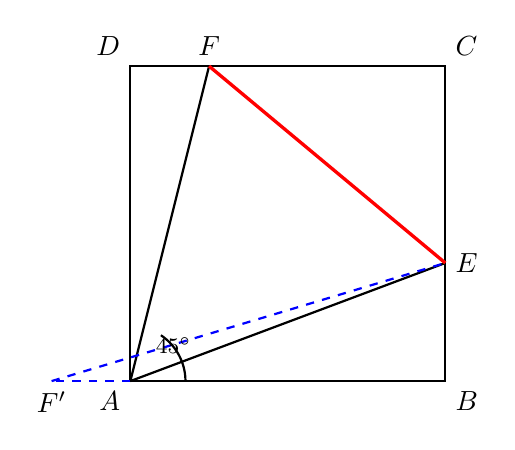
\begin{tikzpicture}[scale=1.0, thick]
  % 正方形 ABCD，边长 4：A 左下、B 右下、C 右上、D 左上
  \coordinate (A) at (0, 0);
  \coordinate (B) at (4, 0);
  \coordinate (C) at (4, 4);
  \coordinate (D) at (0, 4);
  % E 在 BC 上：BE=1.5；F 在 CD 上：DF=1
  \coordinate (E)  at (4, 1.5);
  \coordinate (F)  at (1, 4);
  % F' 在 CB 延长线（B 左侧）上，BF' = DF = 1
  \coordinate (Fp) at (-1, 0);

  \draw (A) -- (B) -- (C) -- (D) -- cycle;

  % 半角的两边
  \draw (A) -- (E);
  \draw (A) -- (F);

  % 旋转后位置（蓝虚线）：△ABF' 复制 △ADF
  \draw[blue, dashed] (A) -- (Fp);
  \draw[blue, dashed] (Fp) -- (E);

  % EF 加粗红色
  \draw[red, very thick] (E) -- (F);

  % 角弧 45°
  \draw (0.7, 0) arc[start angle=0, end angle=56.31, radius=0.7];
  \node at (0.55, 0.45) {\footnotesize $45^\circ$};

  \node[below left]  at (A)  {$A$};
  \node[below right] at (B)  {$B$};
  \node[above right] at (C)  {$C$};
  \node[above left]  at (D)  {$D$};
  \node[right]       at (E)  {$E$};
  \node[above]       at (F)  {$F$};
  \node[below]       at (Fp) {$F'$};
\end{tikzpicture}
\end{document}
